\documentclass[11pt]{beamer}
\usepackage[UTF8]{ctex}
\usepackage[utf8]{inputenc}
\usepackage[T1]{fontenc}
\usepackage{lmodern}
\usepackage{amsmath}
\usepackage{amsfonts}
\usepackage{amssymb}
\usepackage{graphicx}
 \usetheme{CambridgeUS}
 
\usepackage{pdfpages}


%%%%%
\usepackage{longtable}
\usepackage{subfigure}
\usepackage{color}
\usepackage{booktabs}

%% LOGO放右上
\setbeamertemplate{frametitle}
{\begin{beamercolorbox}[wd=\paperwidth]{frametitle}
		\strut\hspace{0.5em}\insertframetitle\strut
		\hfill
		\raisebox{-2mm}{
\includegraphics[width=1cm]{figures/HNUC.jpeg}}
	\end{beamercolorbox}
}

\begin{document}
	\author{郭泰彪}
	\title{区块链原理及应用}
	\subtitle{第1课:区块链思想与技术的起源}
	 \institute{湖南工商大学大数据与互联网创新研究院}
	 \date{2020年9月10日}

	%\date{}
	%\subject{}
	%\setbeamercovered{transparent}
	%\setbeamertemplate{navigation symbols}{}
	\begin{frame}[plain]
		\maketitle
	\end{frame}
	
	\begin{frame}
		\frametitle{目录}
		\tableofcontents[sectionstyle=show,subsectionstyle=show/shaded]
	\end{frame}


\section{导读:谁是中本聪}
\subsection{没人知道比特币的创造者是谁?}
\begin{frame}
	区块链的创世项目Bitcoin(比特币)从2008年由一篇名为《比特币:一种点对点的电子现金系统》被提出,2009年首个比特币网络正式创立,10余年过去了,但Bitcoin的创始人(组织)的真实身份一直不被外人所知,这是区块链世界\textbf{最大的秘密}。
\end{frame}

\subsection{最有可能是中本聪的人}
\begin{frame}
	区块链的创世项目Bitcoin(比特币)从2008年由一篇名为《比特币:一种点对点的电子现金系统》被提出,2009年首个比特币网络正式创立,10余年过去了,但Bitcoin的创始人(组织)的真实身份一直不被外人所知,这是区块链世界\textbf{最大的秘密}。
	
	\hfill
	
	\begin{block}<+->{寻人启事}
	中本聪拥有{\huge 110万}比特币,价值约{\huge 44亿}美元,如果你认识他,或者见到他,请联系我。没有别的,主要是想交个朋友!
	\end{block}	
\end{frame}

\begin{frame}{已知线索}

\begin{figure}
	\centering
	\subfigure{
		\begin{minipage}[ht]{0.7\linewidth}
			\begin{enumerate}
				\footnotesize
				\item 2008年10月31日,
				
				中本聪在“metzdowd.com”网站的密码学邮件列表中发表了一篇论文,题为《比特币:一种点对点式的电子现金系统》;
				\item 2009年1月3日,
				
				中本聪开发出首个实现了比特币算法的客户端程序并进行了首次“采矿”(mining),获得了第一批的50个比特币;
				\item 2010年12月5日, 
				
				中本聪在比特币社区中坚决反对维基解密接受比特币捐款以打破金融封锁,理由是目前比特币还在摇篮中,经不起冲突和争议;
				\item 2010年12月12日,
				
				中本聪在比特币论坛中发表了最后一篇文章,提及了最新版本中的一些小问题;
				
				\item 中本聪消失
				
			\end{enumerate}

		\end{minipage}
	}%
	\subfigure{
		\begin{minipage}[ht]{0.3\linewidth}
{\small 世界上第一个区块}

\tiny
	哈希值:
	
	00000000839a8e6886ab5951d76f411475428afc90947ee320161bbf18eb6048
	
	确认:645,899
	
	高度:1
	
	困难:1.00
	
	默克尔树根:
	
	0e3e2357e806b6cdb1f70b54c3a3a17b6714ee1f0e68bebb44a74b1efd512098
	
	...

		\end{minipage}%	
	}%
\end{figure}
	

\end{frame}

\begin{frame}{候选人:CIA}

	有阴谋论者认为比特币其实是由美国金融机构与政府联手打造的一款骗局工具,目的是以巨大利差引诱投资者巨额投入,再以利差吸取这些投资以平衡美国政府财政。因此中本聪并不是一个人,而是一个小组的代号。这种说法并未得到任何机构或个人的认可,但在反比特币者当中认同度很高。随着近期比特币等加密货币价格的暴跌,这种说法开始在一些比特币持有者当中流传。
\end{frame}

\begin{frame}{候选人:望月新一}
		2012年5月,计算机科学家泰德·尼尔森认为中本聪就是日本数学家望月新一,认为其足够聪明,研究领域包含比特币所使用的数学算法。更重要的是,望月不使用常规的学术发表机制,而是习惯是独自工作,发表论文后让其他人自己理解。然而也有人提出质疑,认为设计比特币所需的密码学并非望月的研究兴趣。望月本人亦予以否认。
\end{frame}

\begin{frame}{候选人:尼克·萨博}
		2013年12月,博客作家Skye Grey通过对中本论文的计量文体学分析得出结论,认为其真实身份是前乔治华盛顿大学教授尼克·萨博。萨博热衷于去中心化货币,还发表过一篇关于“比特黄金”(bit gold)的论文,被认为是比特币的先驱。他也是一个著名的从90年代起就喜欢使用化名的人。
		
		在2011年5月的一篇文章中,萨博谈起比特币创造者时表示:“在我认识的人里面,对这个想法足够感兴趣,并且能付诸实施的,本来只有我自己、戴维(Wei Dai)、哈尔·芬尼三个人,后来中本出现了(假定中本不是芬尼也不是戴维)。”
\end{frame}

\begin{frame}{候选人:多利安·中本}
	最为公众所熟知的猜测发生在2014年3月6日。新闻周刊记者Leah McGrath Goodman发表文章称自己已经找到真正的中本,是一个居住在加利福尼亚州的日裔美国人,名叫多利安·中本,而“哲史”是他出生时的名字。除了名字相同以外,Goodman还找到了一些佐证,其中最有力的一条是,当Goodman在当面采访并提出比特币的问题时,多利安的回答看起来确认了其比特币之父的身份:“我已经不再参与它了,不能讨论它。它已经被转交给其他人。他们现在在负责。我已经没有任何联系。”这段话的真实性亦得到了当时在场的洛杉矶郡警察的确认。
	
	报道被公开后受到了包括比特币社区在内舆论的质疑和批评,但同时也引起了媒体的巨大兴趣。记者们蜂拥而至多利安的住宅外蹲守,甚至追逐他的汽车。然而在后来的正式访谈中,多利安否认了自己与比特币的全部联系,称自己从未听说过,只是误解了Goodman的提问,以为她问的是自己之前从军方承接的保密性工作。
	
	当天晚些时候,中本聪本人也站出来否认。他在P2P基金会的账户在尘封五年之后发了第一条消息,称:“我不是多利安·中本。”
\end{frame}

\begin{frame}{候选人:克雷格·史蒂芬·怀特}
	2015年12月,《连线杂志》报道说澳大利亚学者克雷格·史蒂芬·怀特很有可能是中本聪的本尊。同时也指出,也许只是他精心设计的一个高明的骗局想让我们相信他就是中本聪本人。直到2016年5月2日,澳大利亚企业家克雷格·史蒂芬·怀特公开承认自己就是发明比特币的中本聪,首度有人公开承认。其证据是中本聪的加密签名档,但被质疑该档只要是稍微高端一点的黑客都能在暗网中找到下载,早就在不少电脑高手圈流传,另一证据是早期第1及第9区块比特币地址的私钥,但此私钥如果是早期比特币开发人员或其亲近者都有可能拿到。
	
	最关键证明是导入比特币至2009年的比特币第一笔交易地址,该地址被视为是中本聪所有,并要求表演汇回,BBC记者将0.017个比特币导入,但最终没有汇回。BBC刊登出和他的访谈片段,自称他就是比特币发明者。但克雷格声明与证据的真实性受到普遍的质疑,在最后阶段要求演示关键证据时,克雷格拒绝并发布了一篇顾左右而言他的博客文章。
\end{frame}

\begin{frame}{候选人:其他}
\begin{enumerate}
	\small
	\item 芬兰经济社会学家Dr Vili Lehdonvirta及爱尔兰密码学研究生Michael Clear。两人分别否认。
	\item 德国及美国研究人员Neal King、Vladimir Oksman和Charles Bry。他们曾共同申请注册一项与比特币相关的专利,而比特币项目官方网站的域名bitcoin.org恰好注册于专利申请提交之后的第三天。三人均否认此猜测。
	比特币基金会首席科学家Gavin Andresen、比特币交易平台Mt. Gox创始人Jed McCaleb,或某个政府机构。
	\item 美国企业家及安全研究员Dustin D. Trammell,但他公开否认。
	\item 也有人认为Satoshi Nakamoto的名字实际上是四家公司名字的组合,包括三星(Samsung)、东芝(Toshiba)、中道(Nakamichi)和摩托罗拉(Motorola),暗示着比特币其实是这四家公司联手开发并以Satoshi Nakamoto,即“中本聪”的化名来发表。
\end{enumerate}
\end{frame}

\begin{frame}{没人知道谁是中本聪}
		\centering
		没人知道谁是中本聪\\
		中本聪非常注重隐私
\end{frame}

\subsection{比特币白皮书概览}
\begin{frame}{比特币白皮书截图}
	\centering
	\includegraphics[page=1,width=0.8\textwidth]{figures/BC101.pdf}
\end{frame}

\begin{frame}{比特币白皮书引注概况}
	\centering
	\includegraphics[page=2,width=0.8\textwidth]{figures/BC101.pdf}
\end{frame}

\section{密码朋克时代}
\subsection{从赛博朋克到密码朋克}
\begin{frame}{赛博朋克的含义}
	赛博朋克,将"cyber"(计算机的)和“punk”(朋克)进行组合,形成了以“计算机网络控制”为绝对核心,带有“反乌托邦精神和悲剧色彩”的全新流派。
	
	赛博朋克涵盖了黑客、虚拟实境、人工智能(AI)、都市拓张、贫富差距等话题。
\end{frame}

\begin{frame}{赛博朋克的相关影视作品}
	\centering
	\includegraphics[width=0.8\linewidth,page=4]{figures/bc101.pdf}
\end{frame}

\begin{frame}{加密朋克宣言对隐私的解释}
	在电子时代,对于开放的社会来说,隐私必不可少。隐私不等同于秘密。隐私是某人不想公之于众的东西。而秘密,是他不想让任何人知道的东西。{\color{red}隐私是一种权利},它让某人有权利决定公开什么,不公开什么。
	
	\hfill
	
	\rightline{——节选自《加密朋克宣言》(1993)}
\end{frame}

\begin{frame}[allowframebreaks]{加密朋克宣言}
	\footnotesize
	在电子时代,对于开放的社会来说,隐私必不可少。隐私不同于秘密。隐私是某人不想公之于众的东西。而秘密,是他不想让任何人知道的东西。{\color{red}隐私是一种权力}。它让某人有权决定公开什么,不公开什么。
	
	如果双方进行某种交易,那么他们各自拥有这一互动的记忆。双方都有权陈述各自关于此次交易的记忆。谁能够禁止他们发言呢?或许有人能够通过立法来禁止,但相比于隐私,言论自由对于开放社会来说甚至更加重要。我们不会试图限制任何言论。如果许多人够在同一个论坛上发言,那么每个人相当于对所有人发言,这样就可以同时积累个人和众人的知识。电子化的交流让这一小组得以实现,即使有人想要禁止小组产生,他也不可能成功。
	
	因为我们渴望隐私,所以我们必须确保交易双方仅获得交易所需的信息。因为任何信息都可能在交易中提及,所以我们必须保证暴露最少的信息。在大多数情况下,个人信息并非必不可少。当我在商店里购买一本杂志,付钱给店员的时候,他没有必要知道我是谁。当我要求我的电子邮件服务商发送和接受消息时,他没有必要知道我在给谁发送信息,我发送了什么,或者别人对我说了什么;他只需要知道如何从这里获得消息,我欠他多少服务费。当我的身份在交易中被服务商暗中获取了,我就没有了隐私。我无法再选择性的披露我的信息;我只能被迫一直处于暴露的状态。
	
	由此可见,{\color{red}保护开放社会中的隐私需要匿名的交易系统}。迄今为止,现金交易系统是最好的匿名交易系统。匿名交易系统并非秘密交易系统。当且仅当他们想要这么做时,匿名系统允许个体披露他们的身份,这是隐私的实质。
	
	开放社会中的隐私同样需要密码学。当我发言时,我只想让我指定的听众听到它。当我发言的内容全世界都可以听到时,我就丧失了隐私。加密象征了意味着对隐私的要求,用弱密码加密意味着对隐私要求不高。再者,当披露默认情况下为匿名的个人身份时,为了保证这个披露真实可靠,我们需要{\color{red}密码学的数字签名}。
	
	我们不能奢望政府、企业、或者其他庞大、匿名的组织出于他们的仁慈来授予我们隐私权。评价我们会对他们有利,并且我们应该认为他们确实会这么做。要抵抗他们的言论就是要对抗信息的性质。信息不止想要免费,而且渴望免费。信息会扩展到所有可能的储存空间。信息是谣言的兄弟,它更年轻,更强壮;与流言相比,信息传播得更快,有更多的角度,包含更多的知识,然而给出的结论更少。
	
	如果想要获得隐私权,我们必须捍卫它。{\color{red}我们必须联合起来,创造可以处理匿名交易的系统}。几个世纪以来,人们已经通过低语、夜幕、信封、紧密的房门、秘密的手语,以及邮递员来保护自己的隐私。过去的技术无法支持可靠的隐私,但电子技术可以。
	
	{\color{red}我们,密码朋克,致力于构建匿名系统。为了捍卫我们的隐私,我们用密码学,用匿名邮件转发系统,用数字签名,用电子货币}。
	
	密码朋克写代码。我们认识到,需要有人编写软件来保护隐私,而且我们无法在有人没有隐私的情况下获得隐私,所以我们将会开发这些软件。届时,我们将开源我们的代码,让我们的密码朋克战友们可以使用它。我们的代码对全球,任何使用它的人免费。如果你要封杀我们写的软件,我们不在乎。{\color{red}我们清楚,软件是无法被销毁的,彻底的分布式系统永不停机}。
	
	密码朋克们谴责对于密码学的控制,因为加密从根本上是一种私人行为。加密实际上是从公共领域抹掉我们的信息。即使是禁止密码学的法律也只能在一国的疆界内生效,在国家暴力机器所能控制的范围内肆虐。{\color{red}密码学将不可避免地扩散到全球,同样,它创造的匿名交易系统也将如此}。
	
	要使隐私权的意识广为传播,它必须成为社会契约的一部分。{\color{red}人们必须联合起来,为了共同的利益,合力去部署这些系统}。隐私权的未来,取决于人们在社会中的合作。我们,密码朋克,思你所思,忧你所忧,并且希望与你携手,不再自我欺骗。我们绝不会因为有谁反对,放弃我们的事业。
	
	密码朋克致力于使网络对隐私更加安全。让我们一起加速向前迈进。
	
	前进。
	
	埃里克·休斯
	
	<hughes@soda.berkeley.edu>
	
	1993年3月9日
	
\end{frame}

\begin{frame}{密码朋克宣言与比特币白皮书对比}
	% Please add the following required packages to your document preamble:
	% \usepackage{booktabs}
	\begin{table}[]
		\begin{tabular}{@{}lll@{}}
			\toprule
			话题和技术     & 密码朋克宣言 & 比特币白皮书\footnote{比特币白皮书中文翻译版:https://bitcoin.org/files/bitcoin-paper/bitcoin\_zh\_cn.pdf} \\ \midrule
			隐私保护       & Y      & Y      \\
			去中介化      & Y      & Y      \\
			匿名交易      & Y      & Y      \\
			数字签名      & Y      & Y      \\
			大型机构不可信 & Y   & Y \\
			点对点系统     & Y      & Y      \\
			电子货币      & Y      & Y      \\
			开源代码      & Y      & Y      \\
			激励机制      & Y      & Y      \\ 
			社会实验      & N      & Y      \\
			\bottomrule
		\end{tabular}
		\caption{密码朋克宣言与比特币白皮书涉及的话题对比}
		\label{tab:ccb}
	\end{table}
\end{frame}

\section{数字经济时代的隐私保护}

\subsection{数据的价值}

\subsection{什么是隐私}

\begin{frame}{什么是隐私?}
	\centering	
	{\huge ?}
\end{frame}

\begin{frame}{什么是隐私?}
	\centering
	{\large 隐私=你不想让别人知道的信息}
\end{frame}

\begin{frame}{隐私泄露案例分析:脸书数据门}

	\begin{minipage}[t]{0.5\linewidth}
	\footnotesize
	\begin{enumerate}
		\item 2018/03/17 
		
		媒体曝光Facebook上超5000万用户信息在用户不知情的情况下,被政治数据公司“剑桥分析”获取并利用
		\item 2018/03/26 
		
		扎克伯格登报道歉
		\item 2018/03/30 
		
		Facebook终止与大数据企业合作
		\item 2018/04/05 
		
		脸书隐私泄露人数升至8700万
		\item 2018/04/10 
		
		扎克伯格国会听证证词
		\item 2018/04/11 
		
		扎克伯格二度接受国会质询
	\end{enumerate}
	%		\begin{figure}
	%			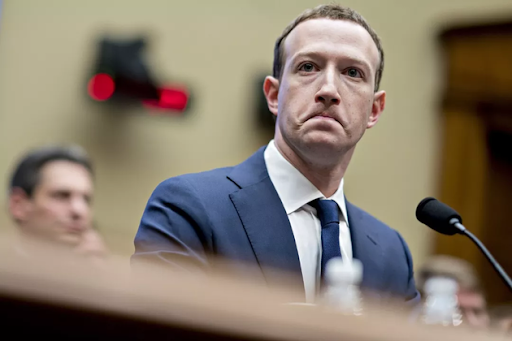
\includegraphics[width=0.8 \linewidth]{figures/privacy/zake.png}
	%		\end{figure}
\end{minipage}%
	\begin{minipage}[t]{0.4\linewidth}
		\begin{figure}
			\centering
			\subfigure[脸书隐私泄露听证会]{
				\begin{minipage}[b]{0.8\linewidth}
					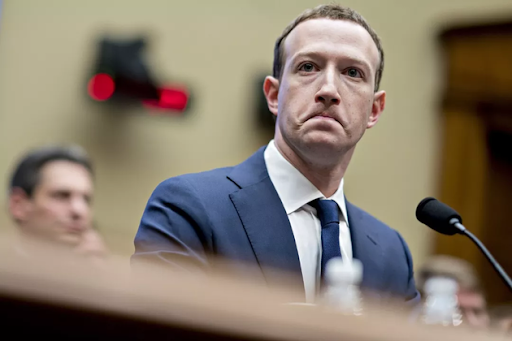
\includegraphics[width=\linewidth]{figures/privacy/zake.png}
				\end{minipage}%
			}
			\subfigure[脸书开始强调隐私]{
				\begin{minipage}[b]{0.8\linewidth}
					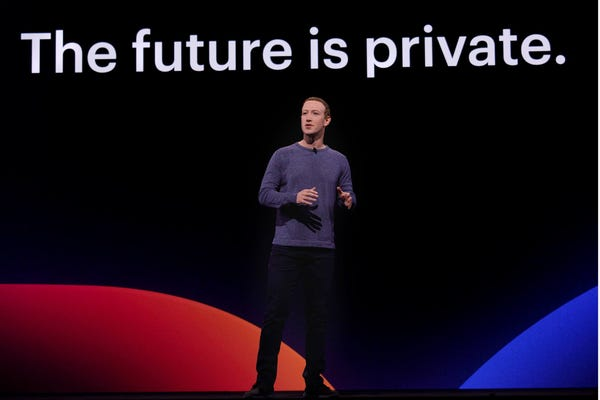
\includegraphics[width=\linewidth]{figures/privacy/zakePrivacy.jpeg}
				\end{minipage}%
			}
		\end{figure}
	\end{minipage}%
\end{frame}


\begin{frame}[allowframebreaks]{隐私泄露案例分析:脸书数据门操纵英国脱欧}
	
	\begin{minipage}[t]{0.7\linewidth}

主角:英国数据公司“剑桥分析”(Cambridge Analytica)

通过Facebook的用户数据等资料,构建了一个“工业规模”的操纵选民行为的全球基础设施网络。

\begin{itemize}
	\item 初级手段:
		\begin{itemize}
			\item 制造假新闻在脸书上传播;
			\item 机器人水军涨粉控评;
		\end{itemize}
	\item 中级手段:AI换脸换声音,伪造知名人士视频;
	\item 高级手段:AI预测地区政治倾向;
	
	{\tiny 例子:如果一个社区的轿车数量大于皮卡的数量,那么该地区有88%的可能性会投票给民主党。如果皮卡的数量大于轿车,则该选区投票给共和党的可能性是82%。}
		
\end{itemize}

\end{minipage}%
	\begin{minipage}[t]{0.3\linewidth}
		\begin{figure}
			\centering
			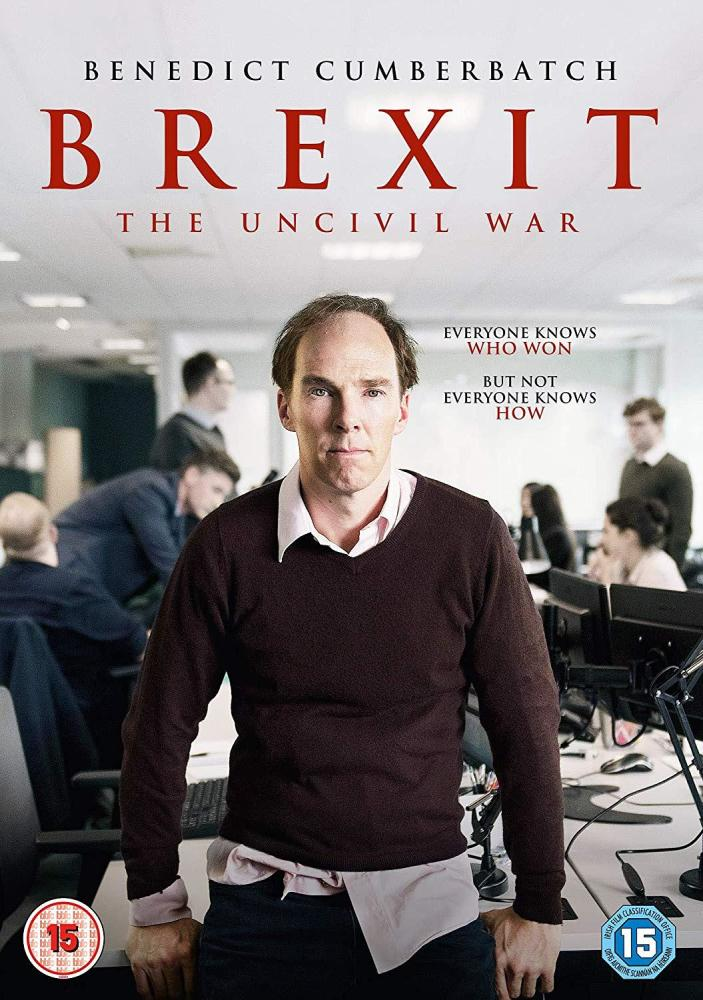
\includegraphics[width=0.7\linewidth]{figures/privacy/brexit.jpeg}
			\caption{《脱欧:无理之战》2019}
		\end{figure}
	\end{minipage}%

\newpage
	\begin{minipage}[t]{0.6\linewidth}
		\begin{figure}
			\begin{itemize}
				\item 点赞
				\item OCEAN分数,心理测量学概念
				\begin{itemize}
					\item 开放度 (openness to experience)
					\item 自律(conscientiousness)
					\item 外向 (extraversion)
					\item 随和 (agreeableness)
					\item 神经质 neuroticism)
				\end{itemize}
				\item 第三方数据,如电视偏好、航空习惯、购物习惯等
			\end{itemize}
			\caption{剑桥分析的个性化广告模型, \quad {\tiny 完整的用户建模大概会采集4000-5000个数据点}}
		\end{figure}
	\end{minipage}%
	\begin{minipage}[t]{0.4\linewidth}
		\begin{itemize}
			\item 揭露了一个事实:我们可以操作公众的意识
			
			\item 武器:人工智能+大数据分析
			
			\item 弹药:社交网络的用户数据
		\end{itemize}
	\end{minipage}%


\newpage

	\centering{
	正在发生:
	
	特朗普和拜登的总统选举之战,谁会赢?
	\begin{figure}
		\centering
		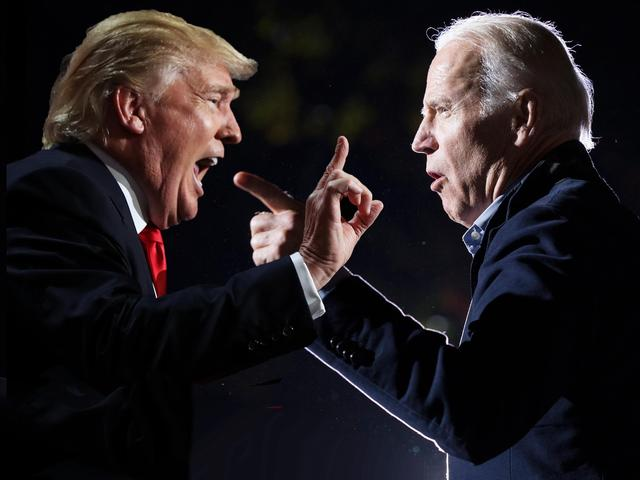
\includegraphics[width=0.6\linewidth]{figures/privacy/turmpbaideng}
		\label{fig:turmpbaideng}
	\end{figure}	
}
	\newpage
	特朗普
	
	\begin{figure}
		\centering
		
		\subfigure{
			\begin{minipage}[t]{0.3\linewidth}
				\centering
				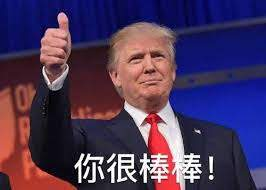
\includegraphics[width=0.6\linewidth,height=0.2\textheight]{figures/privacy/trump/1}\\
				\vspace{0.02cm}
				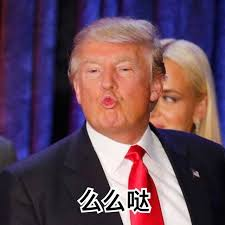
\includegraphics[width=0.6\linewidth,height=0.2\textheight]{figures/privacy/trump/2}\\
				\vspace{0.02cm}
				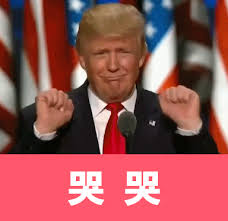
\includegraphics[width=0.6\linewidth,height=0.2\textheight]{figures/privacy/trump/3}\\
				\vspace{0.02cm}
				%\caption{fig1}
			\end{minipage}%
		}%
		\subfigure{
			\begin{minipage}[t]{0.3\linewidth}
				\centering
				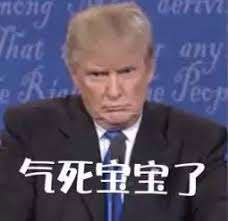
\includegraphics[width=0.6\linewidth,height=0.2\textheight]{figures/privacy/trump/4}\\
				\vspace{0.02cm}
				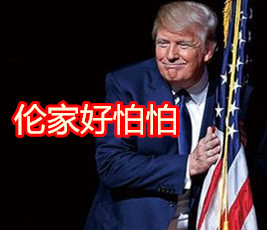
\includegraphics[width=0.6\linewidth,height=0.2\textheight]{figures/privacy/trump/5}\\
				\vspace{0.02cm}
				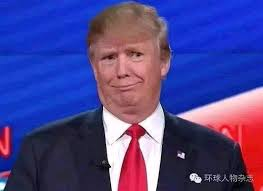
\includegraphics[width=0.6\linewidth,height=0.2\textheight]{figures/privacy/trump/6}\\
				\vspace{0.02cm}
				%\caption{fig1}
			\end{minipage}%
		}%
		\subfigure{
		\begin{minipage}[t]{0.3\linewidth}
			\centering
			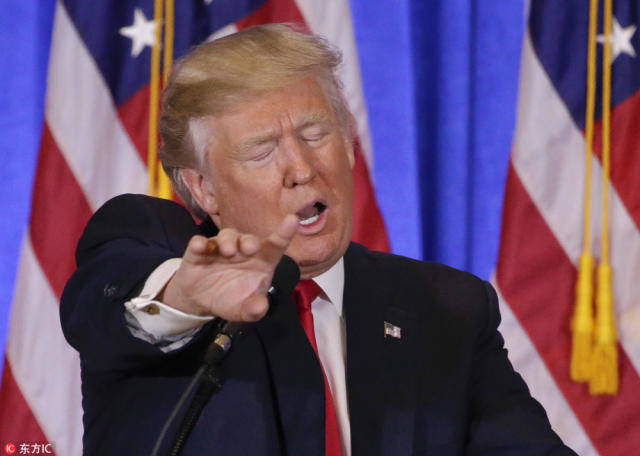
\includegraphics[width=0.6\linewidth,height=0.2\textheight]{figures/privacy/trump/7}\\
			\vspace{0.02cm}
			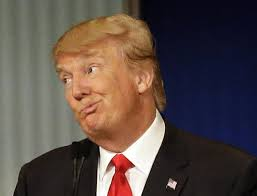
\includegraphics[width=0.6\linewidth,height=0.2\textheight]{figures/privacy/trump/8}\\
			\vspace{0.02cm}
			
\includegraphics[width=0.6\linewidth,height=0.2\textheight]{figures/privacy/trump/9}\\
			\vspace{0.02cm}
			%\caption{fig1}
		\end{minipage}%
	}
	\end{figure}

	\newpage
	
	理由是什么?
	
	\newpage
    
    剑桥分析2.0
    \begin{figure}
    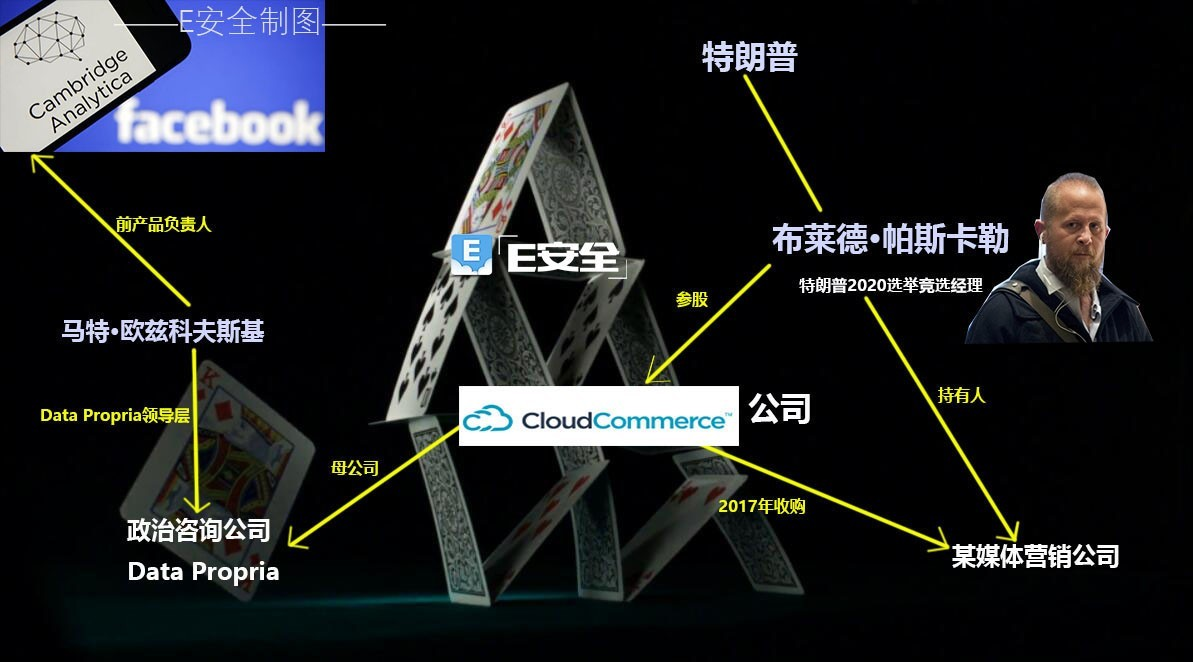
\includegraphics[width=0.6\linewidth]{figures/privacy/ca2}
    \caption{剑桥分析前员工为特朗普2020连任竞选卖力}
    \end{figure}

\end{frame}



\begin{frame}{隐私泄露案例分析:脸书数据门促使隐私保护法规出台}
	
	\begin{minipage}[t]{0.5\linewidth}
		\begin{itemize}
			\item 通用数据保护条例(GDRP)的保护范围
			\begin{itemize}
				\item 个人身份 - {\tiny 电话号码、地址、车牌等}
				\item 生物特征 - {\tiny  指纹、脸部辨识、视网膜扫描、相片等}
				\item 电子纪录 - {\tiny Cookie、IP 位置、移动设备 ID、社群网站活动纪录}
			\end{itemize}
			\item 通用数据保护条例(GDRP)的法规基础
			\begin{itemize}
				\item 被遗忘权
				\item 取用权
				\item 数据可携权 
				\item 隐私始于设计
			\end{itemize}
		\end{itemize}
	\end{minipage}%
	\begin{minipage}[t]{0.4\linewidth}
		\begin{figure}
			\centering
			\subfigure[GDRP]{
				\begin{minipage}[b]{0.8\linewidth}
					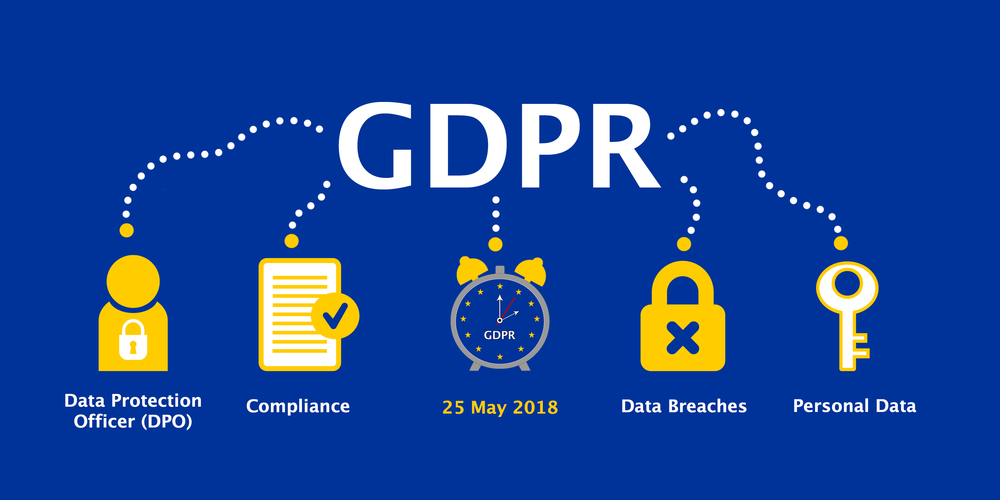
\includegraphics[width=\linewidth]{figures/privacy/gdrp}
				\end{minipage}%
			}
			\subfigure[手机的隐私条款]{
				\begin{minipage}[b]{0.8\linewidth}
					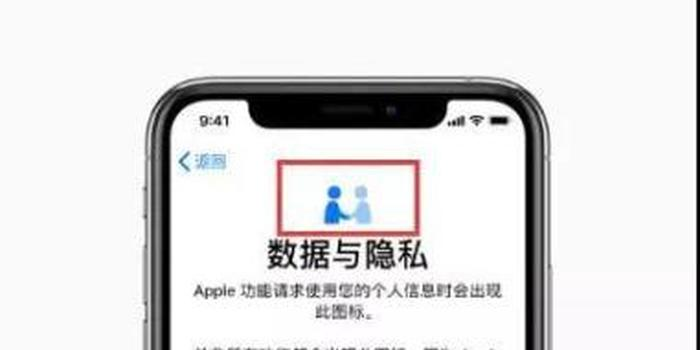
\includegraphics[width=\linewidth]{figures/privacy/Privacyagreement}
				\end{minipage}%
			}
		\end{figure}
	\end{minipage}%
 \end{frame}

\begin{frame}{全球情报收集部门}
	
\begin{minipage}[t]{0.5\linewidth}
 {\footnotesize 英美协定(United Kingdom – United States of America Agreement,缩写为 UKUSA)是一份多边通信条约,让参加国家之间可以共享各项军事与机密情报。参与国包括美国、英国、加拿大、澳洲与新西兰5个英语国家,这5个国家又被称为五眼联盟。最初协定于1946年3月5日签定,其目的在于因应冷战带来的国际情势改变。}

\begin{table}[]
	\centering
	\resizebox{\textwidth}{!}{%
		\begin{tabular}{|l|p{0.5\columnwidth}|p{0.5\columnwidth}|p{0.5\columnwidth}|p{0.5\columnwidth}|}
			\hline
			国家      & 信号情报           & 军事情报               & 安全情报              & 人工情报             \\ \hline
			\# 英国   & 政府通信总部 (GCHQ)  & 英国国防情报局 (DI)       & 军情五处 (MI5)        & 秘密情报局 (MI6)      \\ \hline
			\# 美国   & 美国国家安全局 (NSA)  & 美国国防情报局 (DIA)      & 联邦调查局 (FBI)       & 中央情报局 (CIA)      \\ \hline
			\# 澳大利亚 & 澳大利亚信号局 (ASD)  & 国防情报组织 (DIO)       & 澳大利亚安全情报组织 (ASIO) & 澳大利亚秘密情报局 (ASIS) \\ \hline
			\# 加拿大  & 通信安全机构 (CSE)   & 加拿大武装部队情报司令部 (CDI) & 加拿大安全情报局 (CSIS)   & 加拿大安全情报局 (CSIS)  \\ \hline
			\# 新西兰  & 政府通讯安全局 (GCSB) & 国防情报安全局 (DDIS)     & 新西兰安全情报局 (SIS)    & 新西兰安全情报局 (SIS)   \\ \hline
		\end{tabular}%
	}
	\caption{UKUSA相关情报部门}
	\label{tab:情报部门}
\end{table}
\end{minipage}%
\begin{minipage}[t]{0.4\linewidth}
	\begin{figure}
		\centering
		\subfigure[UKUSA]{
			\begin{minipage}[b]{0.5\linewidth}
				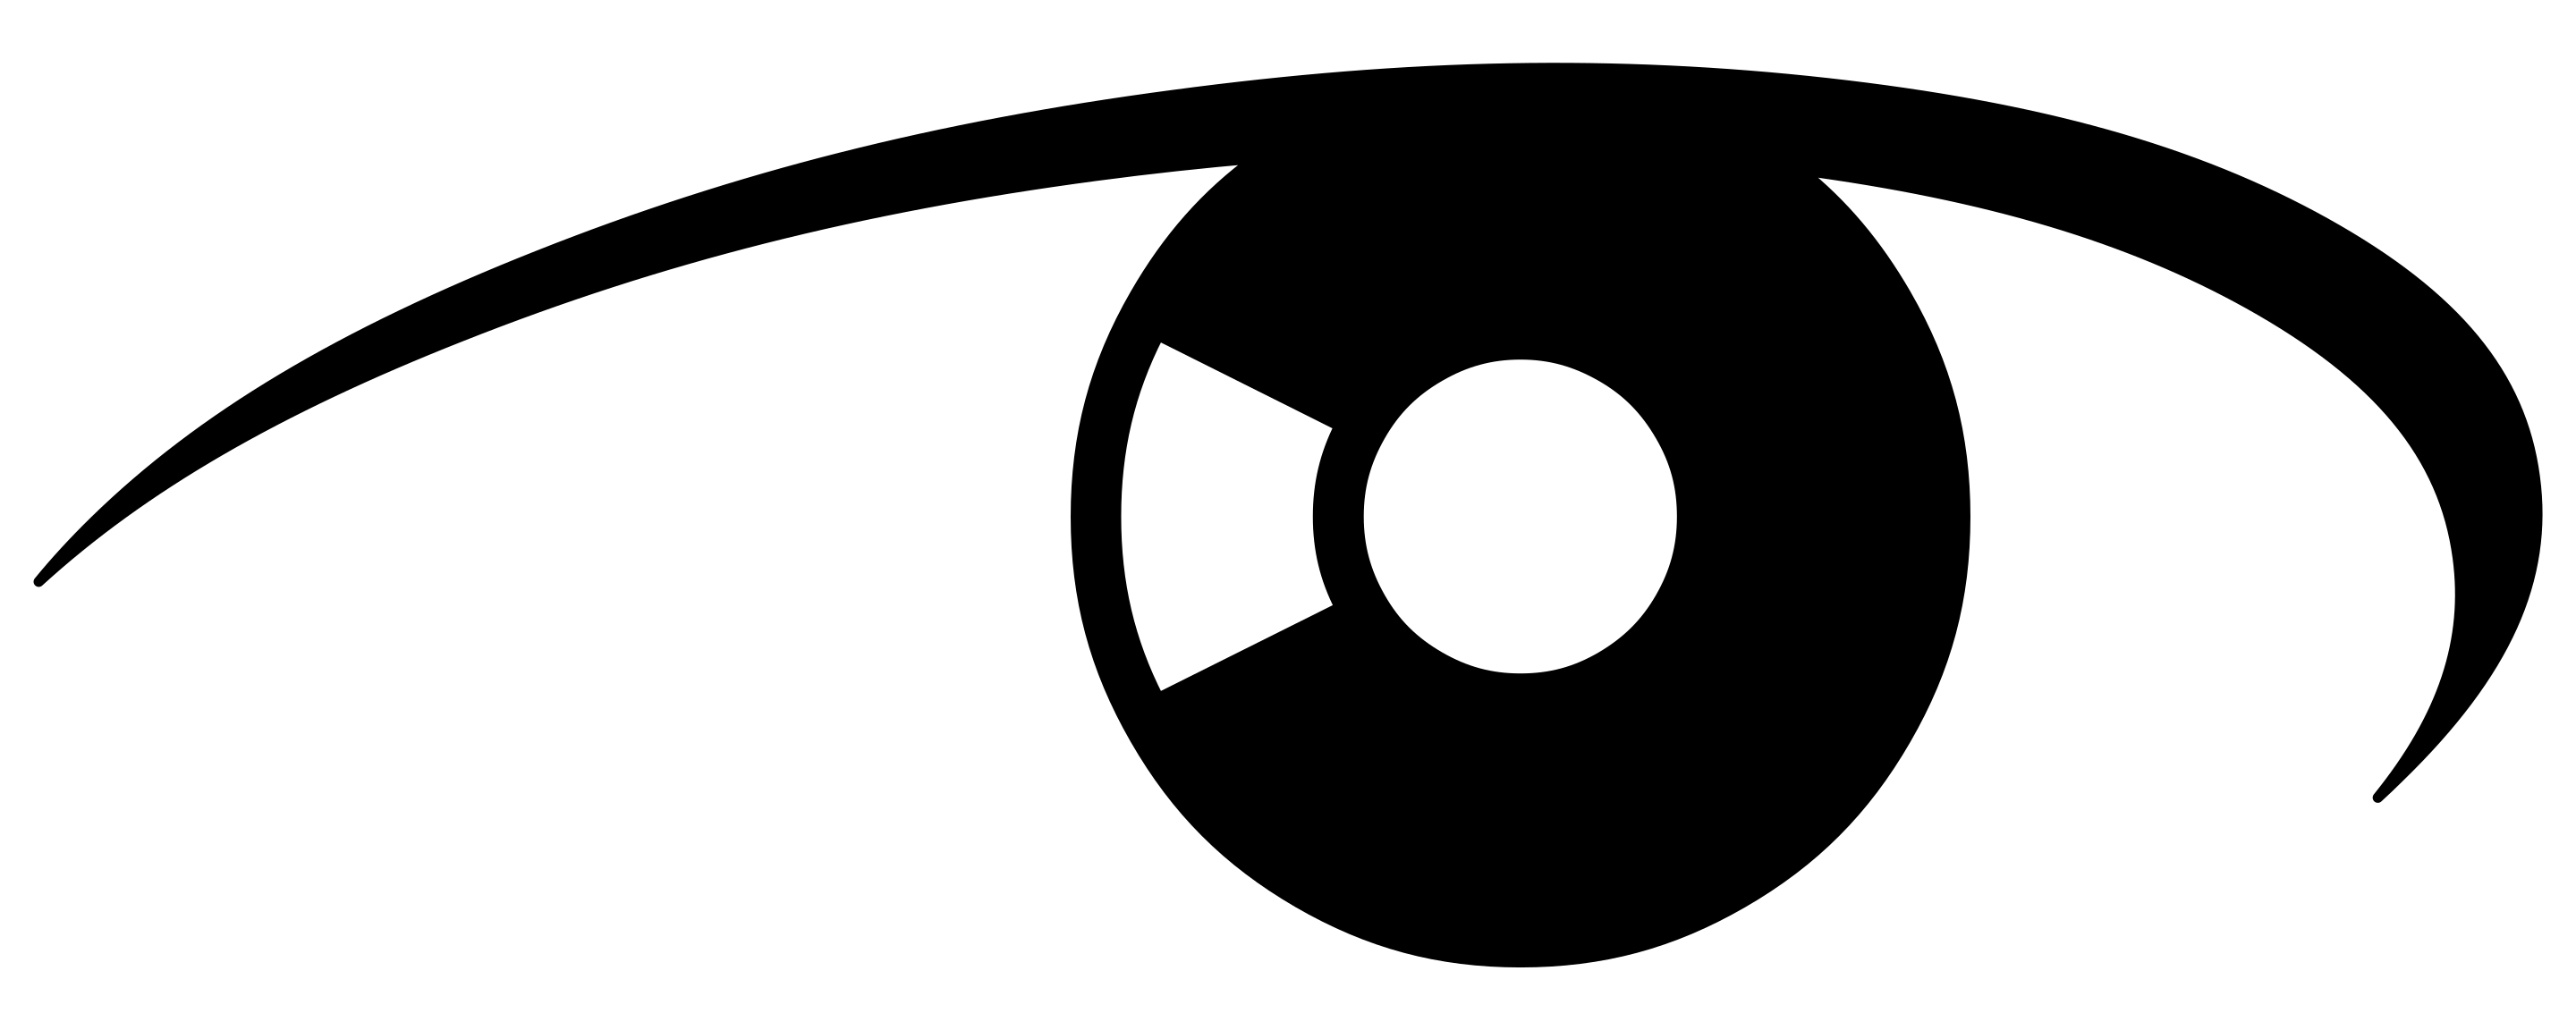
\includegraphics[width=\linewidth]{figures/privacy/Stylizedeye.png}
			\end{minipage}%
			\begin{minipage}[b]{0.5\linewidth}
				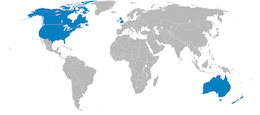
\includegraphics[width=\linewidth]{figures/privacy/UKUSA.png}
			\end{minipage}%
		}
		
		\subfigure[斯诺登]{
			\begin{minipage}[b]{0.4\linewidth}
				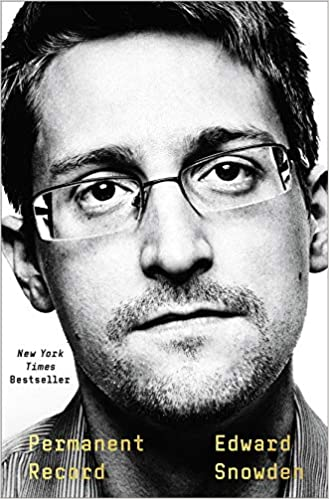
\includegraphics[width=\linewidth]{figures/privacy/Snowden.jpg}
			\end{minipage}%
		}
	\end{figure}
\end{minipage}%
\end{frame}


\subsection{保护隐私的技巧}
	
	\begin{frame}{保护隐私的技巧}
		\centering
		https://cybermagicsec.github.io/privacytools-zh/
	\end{frame}

\section{比特币白皮书原文解析}

\subsection{比特币所用技术族谱}

\begin{frame}[allowframebreaks]{比特币所用技术族谱}
	\centering
	\includegraphics[page=7,width=0.8\textwidth]{figures/BC101.pdf}
	
	\includegraphics[page=8,width=0.8\textwidth]{figures/BC101.pdf}
	
	\includegraphics[page=9,width=0.8\textwidth]{figures/BC101.pdf}
	
	\includegraphics[page=10,width=0.8\textwidth]{figures/BC101.pdf}
	
	\includegraphics[page=11,width=0.8\textwidth]{figures/BC101.pdf}
	
	\includegraphics[page=12,width=0.8\textwidth]{figures/BC101.pdf}
	
	\includegraphics[page=13,width=0.8\textwidth]{figures/BC101.pdf}
	
	\includegraphics[page=14,width=0.8\textwidth]{figures/BC101.pdf}
	
	\includegraphics[page=15,width=0.8\textwidth]{figures/BC101.pdf}
	
	\includegraphics[page=16,width=0.8\textwidth]{figures/BC101.pdf}
\end{frame}

\begin{frame}{比特币白皮书引注概况}
	\centering
	\includegraphics[page=2,width=0.8\textwidth]{figures/BC101.pdf}
\end{frame}

\begin{frame}{密码朋克:从未远去}
	\centering
	\includegraphics[page=17,width=0.8\textwidth]{figures/BC101.pdf}
\end{frame}

%{
%	\setbeamercolor{background canvas}{bg=}
%	\includepdf[pages=7-]{figures/BC101.pdf}
%}





\begin{frame}{想了解更多关于比特币的信息?}
	\centering
比特币社区,包含比特币的百科和开发文档及论文:

https://bitcoin.org/zh\_CN/

\hfil

比特币区块浏览器,试试寻找第一个区块吧:

https://www.blockchain.com/zh/explorer

\end{frame}

\section*{谢谢聆听}

\begin{frame}
	\begin{minipage}[t]{0.5\linewidth}
		\begin{center}
			\begin{figure}
				\vspace{10pt}
				
				{\Huge 谢谢聆听}
				
				\vspace{30pt}
				郭泰彪
				
				\vspace{10pt}
				{\tiny 湖南工商大学大数据与互联网创新研究院}
			\end{figure}
			\begin{figure}
				
			\end{figure}
		\end{center}
	\end{minipage}%
	\begin{minipage}[t]{0.4\linewidth}
		\begin{figure}
			\centering
			\texttt{blockchain101}
			
			
\includegraphics[width=0.6\linewidth]{figures/blockchain101qrcode}
			
			{\footnotesize \texttt{Star| Fork| Issue}}
		\end{figure}
	\end{minipage}%
\end{frame}

\end{document}